%!TEX TS-program = xelatex
\documentclass[]{friggeri-cv}

\usepackage{afterpage}
\usepackage{hyperref}
\usepackage{color}
\usepackage{xcolor}
\usepackage[percent]{overpic}

\ifxetex
  \usepackage{fontspec}
  \usepackage[spanish]{babel}
\else
  \usepackage[T1]{fontenc}
  \usepackage[utf8]{inputenc}
  \usepackage[spanish]{babel}
  \usepackage{lmodern}
\fi

\hypersetup{
    pdftitle={},
    pdfauthor={},
    pdfsubject={},
    pdfkeywords={},
    colorlinks=false,       % no lik border color
   allbordercolors=white    % white border color for all
}
\addbibresource{bibliography.bib}
\RequirePackage{xcolor}
\definecolor{pblue}{HTML}{131A28}

\begin{document}
\header{José Gregorio}{Rincón}
      {Ingeniero Catastral y Geodesta}
      
% Fake text to add separator      
\fcolorbox{white}{gray}{\parbox{\dimexpr\textwidth-2\fboxsep-2\fboxrule}{%
.....
}}

% In the aside, each new line forces a line break
\begin{aside}
  \section{Dirección}
    Calle 25F \#33-32
    111321, Bogotá, Colombia
    ~
  \section{Celular}
    +57 319 240 5609
    ~
  \section{eMail}
    \href{mailto:jgregoriorincon@gmail.com}{jgregoriorincon@\\gmail.com}
    ~
  \section{Tarjeta Profesional}
    25222-314854 CND
    ~ 
  %\section{Web \& Git}
   % \href{http://www.carminebenedetto.net}{carminebenedetto.net}
   % \href{https://bitbucket.org/neoben}{bitbucket.org/neoben}
    %\href{https://github.com/jgregoriorincon}{github.com/jgregoriorincon}
    %~
  \section{Programación}
    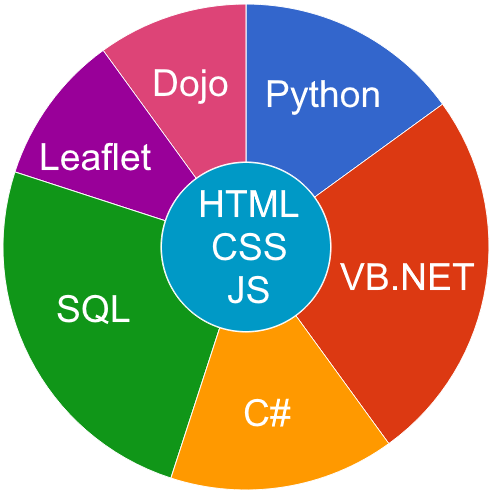
\includegraphics[scale=0.30]{img/Skill_Programacion.png}
    ~
  \section{SIG    }
    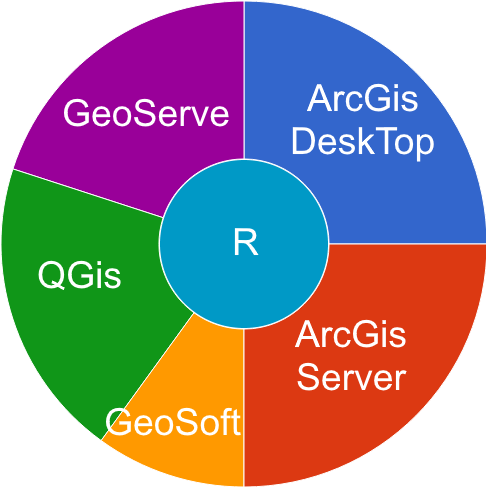
\includegraphics[scale=0.30]{img/Skill_SIG.png}
    ~
  \section{Sistemas Operativos}
  ~
    \textbf{GNU/Linux}
\includegraphics[scale=0.40]{img/2stars.png}
    \textbf{Unix}
\includegraphics[scale=0.40]{img/3stars.png}
    \textbf{MacOS}
\includegraphics[scale=0.40]{img/5stars.png}
    \textbf{Windows}
\includegraphics[scale=0.40]{img/5stars.png}
    \textbf{Citrix}
\includegraphics[scale=0.40]{img/2stars.png}\textbf{}
    ~
\end{aside}

\section{Perfil}
\emph{Amplia experiencia en proyectos de implementación e integración de Sistemas de Información, en especial con información geográfica (ESRI ArcGIS – OpenSource), generación de metodologías orientadas a la solución de problemas espaciales y administración de datos alfanuméricos y geográficos así como con aplicaciones personalizadas. Análisis y procesamiento de datos sociales, geofísicos y espaciales usando técnicas geoestadísticas. Modelamiento y Desarrollo de Bases de Datos Espaciales y Alfanuméricas.}
\\

\section{Experiencia Profesional}
\begin{entrylist}
    \entry
        {2016}
        {Asistente de Investigación}
        {\href{http://www.umng.edu.co/}{Universidad Militar Nueva Granada, Colombia}}
        {Apoyo en la investigación de modelos de ciudades 3D y su publicación con servicios web.\\}
    \entry
        {2012 - 2015}
        {Analista de Datos Geofísicos}
        {\href{http://www2.sgc.gov.co/}{Servicio Geológico Colombiano, Colombia}}
        {Apoyo en la generación del Mapa Tectónico de la cuenca del Valle Medio del Magdalena. Generación del mapa de profundidad de Mohorovicic. Apoyo en la generación del Mapa de la Profundidad de la Isoterma de Curie para Colombia v0 usando el método de Spector y Grant. Apoyo en la generación de cartografía magnetométrica y desarrollo de aplicaciones GIS. Contratos 242/2012, 1068/2012, 276/2013, 212/2014 y 121/2015.\\}
    \entry
        {2011 - 2014}
        {DBA Geográfico}
        {\href{http://www.igac.gov.co/igac}{IGAC, Colombia}}
        {Administración de Bases de Datos Geográficas para la subdirección de Cartografía y Administración del Sistema SIGOT para el GIT de Planeación. Contratos 9601/2011, 10650/2012, 12368/2013 y 14529/2014.\\}
    \entry
        {2011 - 2011}
        {DBA y Desarrollador Web}
        {Enésima Ltda., Colombia}
        {Programación de la Base de Datos SQL Server 2008 para el sistema de Información Inmobiliaria de la Caja Promotora de Vivienda Militar y Policía (CAPROVIMPO) – RUCIV.\\}
    \entry
        {2004 - 2011}
        {Coordinador SIG, DBA y Desarrollador Web}
        {\href{http://www.eninco.com.co/es/index.php?lang=en}{Eninco Ltda., Colombia}}
        {Participación directa en la ejecución, planeación, desarrollo y puesta en producción de proyectos con diferentes entidades, p.ej.:
        \begin{itemize}
            \item Dirección de Derechos Humanos del Ministerio de Justicia y del Interior.
            \item Unidad Administrativa Especial de Catastro Distrital Bogotá.
            \item Planeación Distrital Bogotá.
            \item Acción Social de la Presidencia de la República.
            \item Empresas Públicas de Medellín (EPM).
            \item Corporación Autónoma Regional de Cundinamarca (CAR).
            \item Órgano de Normalización Técnica - Costa Rica
            \item Generación del Catastro y Mapa Tenencial de la Región Metropolitana de Panamá (Zona 4) para el PRONAT - Panamá
        \end{itemize}
        }
\end{entrylist}     

\let\thefootnote\relax\footnote{\enquote{Somewhere, something incredible is waiting to be known} --- Carl Sagan}

\newpage

\begin{aside}
~
~
~
  \section{SGBD}
  ~
    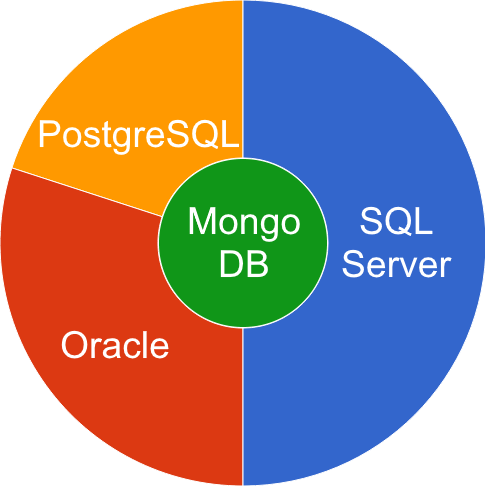
\includegraphics[scale=0.30]{img/Skill_BD.png}
    ~
  \section{Personalidad}
  ~
    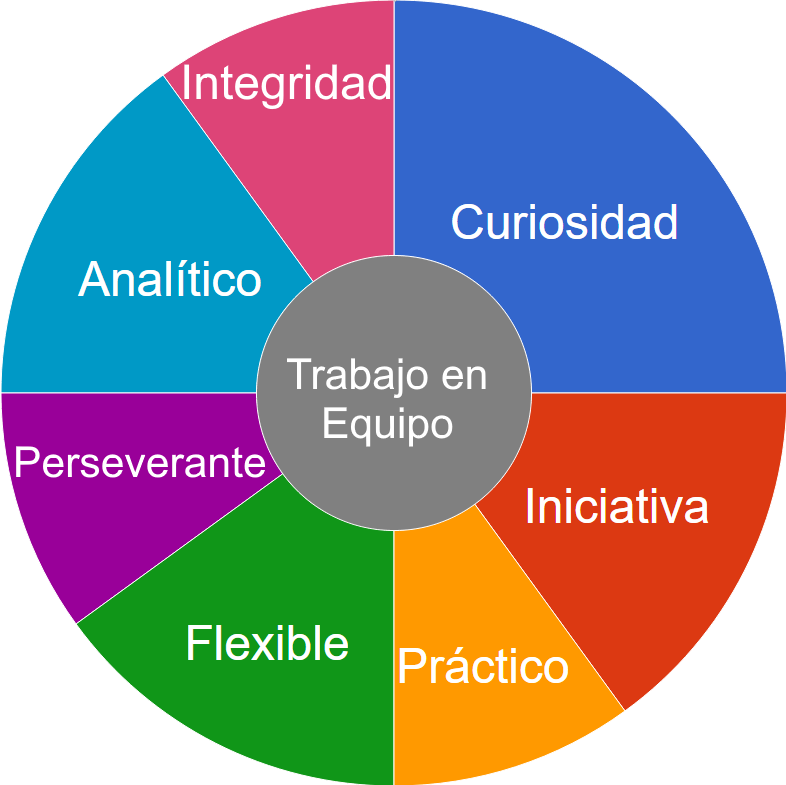
\includegraphics[scale=0.19]{img/Skill_Personal.png}
    ~
  \section{Idiomas}
    \textbf{Español}
\includegraphics[scale=0.40]{img/5stars.png}
    \textbf{Inglés}
\includegraphics[scale=0.40]{img/2stars.png}
\end{aside}

\section{\phantom{Experiencia Profesional (Continuación)}}
\begin{entrylist}
    \entry
        {2002}
        {Desarrollador GIS}
        {\href{http://www.ideam.gov.co/}{IDEAM, Colombia}}
        {Diseño, Implementación y Programación de Modelos Ambientales para la subdirección de Geomorfología y Suelos del Instituto de Meteorología y Medio Ambiente.\\}
    \entry
        {2001 - 2003}
        {QC Metadatos NTC-4611}
        {Tempra Energy Services Ltd., Colombia}
        {Control de Calidad de imágenes escaneadas y Captura de Metadatos sobre la Norma NTC-4611 de los Datos Geocientificos de Exploración y Producción de Ecopetrol.\\}
    \entry
        {1998 - 2000}
        {Coordinador de Sistemas y DBA Oracle 7}
        {Bonvel Ltda., Colombia}
        {Gestión informatica del Proyecto de Preservación Integrada de Historias de pozo y datos Geocientíficos de Exploración y Producción de Ecopetrol.\\}
\end{entrylist}

\section{Educación}
\begin{entrylist}
  \entry
    {En Curso}
    {Especialización en Geomática}
    {\href{http://www.umng.edu.co/web/guest/programas-academicos/facultad-ingenieria/posgrados/especializaciones/especializacion-geomatica}{Universidad Militar Nueva Granada, Colombia}}
    {Áreas Principales: Sistemas de Información Geográfica, Modelamiento de ciudades en 3D, Geoestadística, Sensores remotos.\\
    %\emph{Title of the Thesis: "A Handoff Algorithm based on Link Quality Prediction for Mass Transit Wireless Mesh Networks"      .}\\
    %\emph{Relators: Prof. Enzo Mingozzi, Ing. Carlo Vallati, Prof. Luciano Lenzini.}\\
    }
  \entry
    {2015}
    {Ingeniería Catastral y Geodesia}
    {\href{https://www.udistrital.edu.co/dependencias/tipica.php?id=85}{Universidad Distrital FJDC, Colombia}}
    {Áreas Principales: Geodesia, Sensores Remotos, Planeación municipal, Catastro y Avalúos, Sistemas de Información Geográfica, Programación.\\
    }
\end{entrylist}

%\section{Certifications}
%\begin{entrylist}
%  \entry
%    {02/2013}
%    {Intro to Computer Science}
%    {Udacity. E-learning}
%    {\emph{Building a Python Search Engine}}
%\end{entrylist}



\section{Publicaciones}
W. Quintero, R. A. Ladino, J. G. Rincón, et. al.\\
\textbf{Mapa de la profundidad a la Isoterma de Curie para Colombia v. 0 \\ \scriptsize{(Incluye Mapa Escala 1:3.500.000, Informe Técnico y Anexos Geológicos)}}\\
\emph{Servicio Geológico Colombiano (SGC), Bogotá, Colombia, 2014}
\\
\section{Otros}
\emph{Se autoriza el uso de la información contenida en este Curriculum de acuerdo a las disposiciones previstas en la Ley 1581 de 2012.}
\\
\begin{flushleft}
\emph{\today}
\end{flushleft}

\begin{flushright}
\emph{\large{\\ José Gregorio Rincón Albarracín}}
%
\includegraphics[scale=0.06]{img/Firma.png}
%\begin{overpic}[width=0.5\textwidth,tics=10]{img/Firma.png}
% \put (-10,20) {\emph{\LARGE{José Gregorio Rincón Albarracín}}}
%\end{overpic}

\end{flushright}

\let\thefootnote\relax\footnote{\enquote{Somewhere, something incredible is waiting to be known} --- Carl Sagan}

\end{document}
